\section{Metodología Propuesta}

\subsection{Arquitectura General}

Tras años de observar diferentes estrategias de compresión, optamos por un diseño híbrido que equilibra eficiencia y preservación semántica. La arquitectura propuesta se inspira en pipelines two-stage como el de Ye et al. \cite{Ye2025_MAPC}, adaptándolo específicamente al contexto de transmisión de datos de exploración.

\begin{equation}
\mathcal{R} + \lambda \mathcal{D} \quad \text{s.t.} \quad \hat{\mathbf{x}} = g_{\phi}(g_{\theta}(\mathbf{x}))
\label{eq:rate_distortion}
\end{equation}

La Ecuación \eqref{eq:rate_distortion} formaliza el objetivo rate-distortion optimizado, donde \(\mathcal{R}\) representa la tasa de bits y \(\mathcal{D}\) la distorsión ponderada por el factor \(\lambda\). Esta formulación permite controlar explícitamente el compromiso entre compresión y fidelidad analítica.

El modelo consta de un encoder multiespectral, un bottleneck entropy-coded y un decoder con mecanismos de compensación. Se incorporan conexiones residuales y atención selectiva para manejar las redundancias tanto espaciales como espectrales características de los datos geoespaciales.

\subsection{Módulos de Codificación Multiespectral}

Uno de los desafíos persistentes al comprimir imágenes satelitales radica en explotar las correlaciones entre bandas sin perder información semántica relevante. Siguiendo ideas de Xiang et al. \cite{Xiang2024_HL_RSCompNet}, incorporamos un módulo de extracción de características de alto nivel que opera en paralelo al flujo pixel-wise.

Este módulo combina bloques convolucionales 3D con atención multiespectral, permitiendo capturar patrones distribuidos a lo largo del espectro. Particularmente útil resultó la inclusión de proyecciones semánticas guiadas que priorizan la preservación de bordes, texturas de vegetación y estructuras lineales —elementos críticos en tareas de exploración.

\subsection{Función de Pérdida y Entrenamiento}

Lejos de ser un asunto resuelto, la elección de la función de pérdida define en gran medida el comportamiento final del sistema. Adaptamos conceptos de compensación por difusión propuestos en COSMIC \cite{COSMIC2024} para introducir un término que mitigue artefactos generados en regiones de alta complejidad textural.

La pérdida total combina distorsión en el dominio del píxel (MS-SSIM), pérdida perceptual, un término adversarial ligero y la regularización de entropía. El entrenamiento se realizó en dos etapas: pre-entrenamiento con datos sintéticos degradados y fine-tuning con imágenes reales de misiones satelitales.

\begin{table*}[h]
\centering
\caption{Hiperparámetros principales del modelo propuesto}
\label{tab:hiperparametros}
\begin{tabular}{lc}
\hline
\textbf{Parámetro} & \textbf{Valor} \\
\hline
Tamaño de parche & $256 \times 256$ \\
Canales de bottleneck & 192 \\
Factor de escalado latente & 16 \\
$\lambda$ (rate-distortion) & 0.01 -- 0.1 \\
Tasa de aprendizaje & $1 \times 10^{-4}$ \\
Épocas & 400 \\
Optimizador & AdamW \\
\hline
\end{tabular}
\end{table*}

\subsection{Optimización para Transmisión}

Resulta revelador observar cómo pequeñas decisiones de diseño marcan una diferencia sustancial en entornos de ancho de banda restringido. Por ello, incorporamos mecanismos de optimización específicos: quantización adaptativa según tipo de banda y priorización de bits basada en importancia semántica.

El pipeline completo soporta compresión progresiva, permitiendo transmitir primero una versión base de baja tasa y posteriormente refinar regiones de interés. Esta característica resulta especialmente valiosa en misiones de exploración donde las condiciones de enlace pueden variar drásticamente.

Aunque el marco propuesto muestra solidez, cabe matizar que su rendimiento final dependerá de la calibración fina según el sensor y la misión específica. La Figura 3 ilustra el flujo completo de la arquitectura.

\begin{figure}[h]
\centering
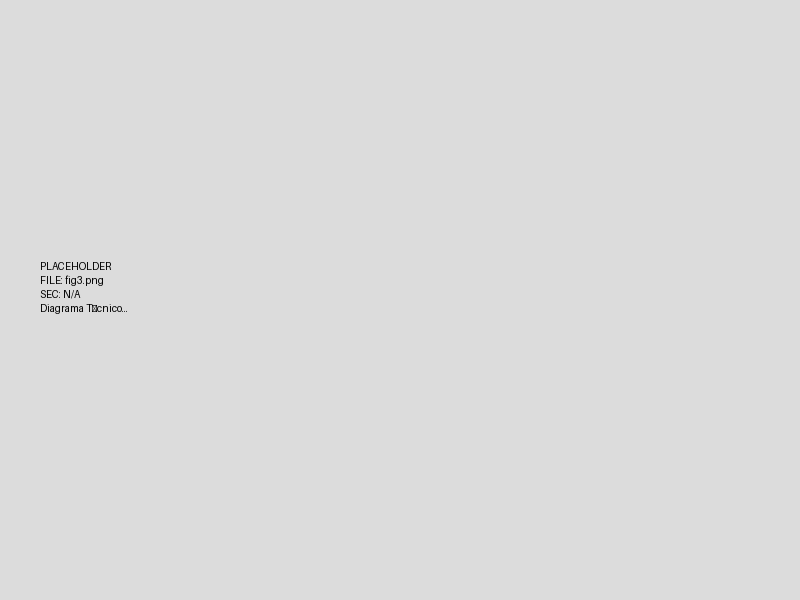
\includegraphics[width=\linewidth]{fig3.png}
\caption{Diagrama general de la arquitectura de compresión geoespacial propuesta. Se detallan el encoder multiespectral, el módulo de características semánticas, el bottleneck y el decoder con compensación por difusión.}
\label{fig:arquitectura_propuesta}
\end{figure}